From \chapter{Chemical Change and Chemical Reactions}


\section{Physical and Chemical Changes}

Changes in state are an example of a physical change. A physical change is a change that only involves rearranging molecules. Chemists also study chemical changes, in which chemical bonds are broken and remade, and molecules change from one kind to another. The following activity may be used with students to illustrate the difference between physical and chemical changes.

\subsection{Physical and Chemical Change}

\subsubsection*{Learning Objectives}
\begin{itemize}
\item{To demonstrate physical and chemical changes of matter experimentally.}
\end{itemize}


\subsubsection*{Materials}
A piece of paper, sugar, spoon, bar magnet, two iron nails, steel wool, kerosene stove and match box.

\subsubsection*{Activity Procedure}
\begin{enumerate}
\item{Take a piece of paper and light it on fire using a match box. Record observations.}
\item{Take a small amount of sugar into the spoon and heat until a clear chemical change is observed. Record  observations.}
\item{Take a bar magnet and rub one nail in one direction only.}
\item{ Place the second (de-magnetized) nail hear the iron fillings. Repeat with the nail that has been rubbed with a magnet.}
\item{Take the magnetized nail and rub it again in the opposite direction and place in iron fillings observe what will happen.}
\end{enumerate}

\subsubsection*{Results and Conclusions}
Burning paper and burning sugar are examples of chemical changes. These means that chemical bonds are broken and remade and new products are formed. But when the nail is rubbed with the bar magnet no chemical bonds are broken or made. The nail becomes magnetized and thus attracts the iron fillings. This is an example of a physical change.

\subsubsection*{Clean Up Procedure}
Collect all the used materials, cleaning and storing items that will be used later. No special waste disposal is required.

\subsubsection*{Discussion Questions}
\begin{enumerate}
\item{Explain the changes in the paper and sugar. Name the type of change.}
\item{Explain the process of rubbing a nail with a bar magnet and what happen when it was rerubbed?}
\item{Why did the two nail behave differently? Name the change that happened in the rubbed nail.}
\end{enumerate}


\section{ Chemical Reactions}
Chemical reactions are chemical changes - chemical bonds are broken and remade. This section includes examples of three common types of reactions - thermal decomposition, binary combination, and precipitation - and activities to guide students to better understand these reactions. There is also a discussion of solubility and another activity to do with students.
\subsection{Precipitation Reaction}
A precipitate reaction is the formation of an insoluble salt by mixing solutions which contain its two components. These reactions are great for teaching students because of the speed and dramatic changes involved. The principles or precipitation are used in many future practicals-including identifying unknowns in qualitative analysis-so this activity is a good introductions to the principles. This activity is best done individually by students or in small groups of 2-3. 

\subsubsection*{Learning Objectives}
\begin{itemize}
\item{To explain the meaning of a precipitation reaction.}
\item{To write chemical equations for the precipitation of insoluble salt.}
\end{itemize}

\subsubsection*{Materials}
Copper sulphate*, soda ash (sodium carbonate)*, beakers*, funnel* and filter paper* (or cloth).

\subsubsection*{Preparation}
\begin{enumerate}
\item{Make a solution of copper sulphate by dissolving about 1 spoonful in 500 mL of water.}
\item{Make a solution of sodium carbonate by dissolving about 1 spoonful in 500 mL of water.}
\end{enumerate}

\subsubsection*{Activity Procedure}
\begin{enumerate}
\item{Take one empty beaker and add about 10 mL of copper sulphate solution.}
\item{To the same beaker add about 10 mL of sodium carbonate solution.}
\item{Filter the mixture and save the insoluble salt.}

\end{enumerate}

\subsubsection*{Results and Conclusions}
When copper sulphate solution is mixed with sodium carbonate a precipitate will form. Copper carbonate is a blue precipitate. This reaction is useful for preparing insoluble salts.
The chemical reactions are 
$$ \ce{CuSO4} _{(aq)} + \ce{Na2CO3}_{(aq)}\longrightarrow \ce{CuCO3}_{(s)} \ce{Na2SO4}_{(aq)} $$

\subsubsection*{Clean Up Procedure}
\begin{enumerate}
\item{Collect all the copper carbonate produced and save for the following pracical (thermal decomposition).}
\item{Collect all the used materials, cleaning and storing items that will be used later. No special waste disposal is required.}
\end{enumerate}

\subsubsection*{Discussion Questions}
\begin{enumerate}
\item{What precipitate is formed in this reaction?}
\item{Write a balanced chemical equation for this reaction.}
\end{enumerate}

\subsubsection*{Notes}
The precipitated copper carbonate should be saved for the following experiment (thermal decomposition).

\subsection{Thermal Decomposition}

Thermal decomposition is when a compound breaks down when heated. Many compounds decompose when heated. Generally there are two products of thermal decomposition -- a gas that leaves the sample and a residue that stays behind. 

\subsubsection*{Learning Objectives}
\begin{itemize}
\item{To explain the meaning of thermal decomposition.}
\item{To observe thermal decomposition of both a salt and an organic compound.}
\item{To write chemical equations for the thermal decomposition a salt.}
\end{itemize}

\subsubsection*{Materials}
Copper carbonate (from the above experiment), citric acid*, metal spoon, heat source.

\subsubsection*{Preparation}
\begin{enumerate}
\item{Dry copper carbonate from the precipitation reaction experiment by leaving it in an open container.}
\end{enumerate}

\subsubsection*{Activity Procedure}
\begin{enumerate}
\item{Place a small amount of copper carbonate in a metal spoon.}
\item{Heat the sample until only a black residue remains.}
\item{Place a small amount of citric acid in a metal spoon.}
\item{Heat the sample until only a black residue remains.}

\end{enumerate}

\subsubsection*{Results and Conclusions}
When copper carbonate is heated, it decomposes to release carbon dioxide. The black reside can be found by subtracting carbon dioxide from the formula for copper carbonate:

$$ \ce{CuCO3} _{(s)} \longrightarrow \ce{CO2}_{(g)} + \ce{CuO}_{(s)} $$

When citric acid is heated, it decomposes twice. First, bubbles of carbon dioxide are released and then, citric acid further decomposes to release water vapor. The black residue at the end of the experiment is solid carbon.

\subsubsection*{Clean Up Procedure}
\begin{enumerate}
\item{Allow spoons to cool before cleaning. Note that hot spoons can burn wood tables.}
\item{Scrap off the residues with another metal spoon and then steel wool. The copper oxide may be saved for future experiments. Neither copper oxide nor solid carbon require special disposal; the solid waste may be put in a pit latine or trash pit.}
\end{enumerate}

\subsubsection*{Discussion Questions}
\begin{enumerate}
\item{What gas is released in the decomposition of copper carbonate?}
\item{Write a balanced chemical equation for this reaction.}
\end{enumerate}

\subsubsection*{Notes}
Thermal decomposition of organic compounds is also called pyrolysis. This is the same process used to make charcoal from plant material.

\subsection{Binary Combination}
Binary combination is the kind of chemical reaction where two elements come together to form a compound. The elements alone are often quite different from the compounds they make up. Iron is a hard, magnetic, silver metal and sulphur is a yellow powder. When heated, the two combine to form iron (II) Sulphide FeS which is a black, insoluble compound. 

This activity gives students a chance to observe a binary combination reaction by heating sulphur and iron together. The students will investigate the properties of the elements before the reaction as well as the final product. Because this activity might lead to the production of a gas that could be harmful in large amounts, it is best done as a teacher demonstration.

\subsubsection*{Learning Objectives}
\begin{itemize}
\item{To demonstrate a binary combination reaction.}
\item{To write a balanced equation for the binary combination of iron and sulphur.}
\end{itemize}

\subsubsection*{Materials}
Sulphur*, steel wool, source of heat*, tea spoon, heating vessel*, bar magnet and aluminium plate.

\subsubsection*{Hazards and Safety}
\begin{itemize}
\item{This reaction produces sulphur dioxide, a poisonous gas. Perform this reaction outside or in a well-ventilated room and stand upwind.}
\item{This experiment involves open flames a bucket of water or sand should be available for fire fighting purposes.}
\end{itemize}

\subsubsection*{Preparation}
Grind the steel wool using a spoon on a hard surface so that fine particles are obtained.

\subsubsection*{Activity Procedure}
\begin{enumerate}
\item{Put half a teaspoon of iron particles in a beaker and add the same amount of sulphur powder. Mix them well.}
\item{Put a bar magnet into the mixture and observe the results.}
\item{Put some iron fillings in the heating vessel, add twice as much sulphur powder to it and mix them well. Heat the mixture until the sulphur powder is gone.}
\item{Again use a bar magnet to try to separate the two components physically from the mixture and record the results.}
\item{To another heating vessel put few iron fillings, add sulphur powder to it and mix them. Heat the mixture strongly for an extended time.}
\item{Use a a bar magnet and to try separate the two components physically from the mixture and record the results. If nothing is observed on the bar magnet, continue heating and try again.}
\end{enumerate}

\subsubsection*{Results and Conclusions}
The mixture of sulphur and iron before heating can easily be separated by physical means because iron has magnetic properties while sulphur does not. When the second mixture is heated, the iron and sulphur combine to form iron (II) sulphide. Because the sulphur and iron are chemically bound together, they cannot be separated by physical means. In the third trial the iron sulphide is heated extensively, liberating the sulphur as sulphur dioxide. This leaves iron metal behind (or an iron oxide) which can be picked up using a magnet.

\subsubsection*{Clean Up Procedure}
Collect all the used materials, cleaning and storing items that will be used later. No special waste disposal is required. Solid waste should not be put in the drain.

\subsubsection*{Discussion Questions}
\begin{enumerate}
\item{What do you understand by the term binary combination?}
\item{Write the equation for the binary combination of Iron and sulphur.}
\item{Why was there no effect of the bar magnet in mixture 2?}
\end{enumerate}

\subsection{Rusting}

Rusting is a chemical reaction similar to combustion which was seen in the first chapter. Chemically rusting is very similar to combustion. Both are examples of a materials undergoing destructive oxidation through reaction with oxygen gas. Iron rusts by reacting with oxygen and water to form a hydrated iron oxide called rust.

This activity is useful for showing students the conditions required for rusting - metal, oxygen (air), and water. After students learn about the requirements of rusting, they can participate in a discussion about how to prevent rusting. This activity should be performed by students working in small groups. The experiment should be started in one period and discussed in the next as at least 24 hours are required for results.
\subsubsection*{Objectives}
\begin{itemize}
\item{To demonstrate the conditions necessary for rusting}
\end{itemize}

\subsubsection*{Materials}
Oil, water, sealed syringes, syringe plungers, iron (non-galvanized) nails, iron wool* and paint.

\subsubsection*{Activity Steps}
\begin{enumerate}
\item{Label 6 sealed syringes with the numbers 1-6}
\item{Place a nail in syringe 1 and fill with water. Leave open to air. This is the control.}
\item{Place a nail in syringe 2 and fill with water. Place the plunger back to seal the syringe to prevent oxygen from entering the shell.}
\item{Place a nail in syringe 3 and cover with oil. Leave open to air.}
\item{Place a nail in syringe 4 and cover with oil. Replace plunger to seal the syringe.}
\item{Place a nail in syringe 5 cover with water. Make an oil layer with a thickness of at least 2 cm.}
\item{Take a nail and paint the nail to cover the metal completely. Now place in syringe 6 and fill with water.}
\begin{figure}[h]
\begin{center}
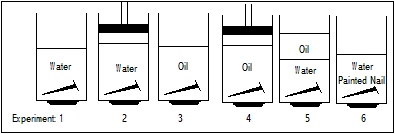
\includegraphics[scale=0.75]{../img/rust-prevention.png}
\caption{Rust Prevention}
\end{center}
\end{figure}


\end{enumerate}


\subsubsection*{Results and Conclusions}  
Syringe 1 is the control experiment. This will be the normal rusting of the iron nail. Syringe 2 now prevents any oxygen from participating in the rusting reaction. This nail should have little or no rust. Syring 3 allows oxygen to encounter the oil for rusting; however, there is no water since it is filled with oil. In addition, oxygen migrates through oil very poorly that also limits the available oxygen for rusting on the surface of the nail. There should be little or no rusting on the nail. Syringe 4 has no oxygen or water available for rusting. This nail should have no rusting. Experiment 5 allows water available to react, but now there is an oil layer. This oil layer prevents oxygen from entering the water layer and rusting the iron nail. This nail should have little or no rust. Syring 6 is much like the control, but since the nail is painted, there is no iron available to react since it is protected by the paint. In each of these experiments, the availability of the iron, oxygen, and water change and the effects of the lack of availability of each component slow down or even prevent the rusting reaction.
\subsubsection*{Clean Up Procedure}
Collect all the used materials, cleaning and storing items that will be used later. No special waste disposal is required.
\subsubsection*{Discussion questions}
\begin{enumerate}
\item{Which nail had the most rust at the end? Which nail had the least?}
\item{What was the purpose of oil in this experiment? What was the function of the plunger?}
\item{Why are ships painted even on surfaces that cannot be seen?}
\end{enumerate}